
%%\documentclass[12pt,preprint]{aastex}

%% manuscript produces a one-column, double-spaced document:

%% \documentclass[10pt,manuscript]{aastex}

%% preprint2 produces a double-column, single-spaced document:
\documentclass[preprint2,iop,numberedappendix]{emulateapj}
%% \documentclass[preprint2,iop]{aastex}

%% \documentclass[preprint2,longabstract]{aastex}

%% \usepackage{ccaption}
%% \captionstyle{\raggedright}
\usepackage[caption=false]{subfig}
\usepackage{amsmath}
\usepackage{footnote}
\bibpunct{(}{)}{;}{a}{}{,} 
\captionsetup{belowskip=12pt,aboveskip=4pt}
\setlength{\textfloatsep}{10pt plus 1.0pt minus 2.0pt}
\newcommand{\dif}{\mathrm{d}}
%% \renewcommand*{\thefootnote}{\fnsymbol{footnote}}

\def\nar{{New~A~Rev.}}          % New Astronomy Review
\def\pasa{{PASA}}               % Publications of the Astron. Soc. of Australia

%% \bibliographystyle{mn2e}
%% \bibliographystyle{apj}

\shorttitle{Foreground signatures in EoR power spectra}
\shortauthors{Thyagarajan et~al.}

\def\ASU{\altaffilmark{1}}
\def\ASUtxt{\altaffiltext{1}{School of Earth and Space Exploration, Arizona State University, Tempe, AZ 85287, USA; e-mail: t\_nithyanandan@asu.edu}}

\def\UW{\altaffilmark{2}}
\def\UWtxt{\altaffiltext{2}{Department of Physics, University of Washington, Seattle, WA 98195, USA}}

\def\RRI{\altaffilmark{3}}
\def\RRItxt{\altaffiltext{3}{Raman Research Institute, Bangalore 560080, India}}

\def\SKASA{\altaffilmark{4}}
\def\SKASAtxt{\altaffiltext{4}{Square Kilometre Array South Africa (SKA SA), Cape Town 7405, South Africa}}

\def\ANU{\altaffilmark{5}}
\def\ANUtxt{\altaffiltext{5}{Research School of Astronomy and Astrophysics, Australian National University, Canberra, ACT 2611, Australia}}

\def\Haystack{\altaffilmark{6}}
\def\Haystacktxt{\altaffiltext{6}{MIT Haystack Observatory, Westford, MA 01886, USA}}

\def\Curtin{\altaffilmark{7}}
\def\Curtintxt{\altaffiltext{7}{International Centre for Radio Astronomy Research, Curtin University, Bentley, WA 6102, Australia}}

\def\USydney{\altaffilmark{8}}
\def\USydneytxt{\altaffiltext{8}{Sydney Institute for Astronomy, School of Physics, The University of Sydney, NSW 2006, Australia}}

\def\CAASTRO{\altaffilmark{9}}
\def\CAASTROtxt{\altaffiltext{9}{ARC Centre of Excellence for All-sky Astrophysics (CAASTRO)}}

\def\MIT{\altaffilmark{10}}
\def\MITtxt{\altaffiltext{10}{Kavli Institute for Astrophysics and Space Research, Massachusetts Institute of Technology, Cambridge, MA 02139, USA}}

\def\CfA{\altaffilmark{11}}
\def\CfAtxt{\altaffiltext{11}{Harvard-Smithsonian Center for Astrophysics, Cambridge, MA 02138, USA}}

\def\Victoria{\altaffilmark{12}}
\def\Victoriatxt{\altaffiltext{12}{School of Chemical \& Physical Sciences, Victoria University of Wellington, Wellington 6140, New Zealand}}

\def\UWisc{\altaffilmark{13}}
\def\UWisctxt{\altaffiltext{13}{Department of Physics, University of Wisconsin--Milwaukee, Milwaukee, WI 53201, USA}}

\def\UMichigan{\altaffilmark{14}}
\def\UMichigantxt{\altaffiltext{14}{Department of Atmospheric, Oceanic and Space Sciences, University of Michigan, Ann Arbor, MI 48109, USA}}

\def\CASS{\altaffilmark{15}}
\def\CASStxt{\altaffiltext{15}{CSIRO Astronomy and Space Science (CASS), PO Box 76, Epping, NSW 1710, Australia}}

\def\Tata{\altaffilmark{16}}
\def\Tatatxt{\altaffiltext{16}{National Centre for Radio Astrophysics, Tata Institute for Fundamental Research, Pune 411007, India}}

\def\NRAO{\altaffilmark{17}}
\def\NRAOtxt{\altaffiltext{17}{National Radio Astronomy Observatory, Charlottesville and Greenbank, USA}}

\def\UMelbourne{\altaffilmark{18}}
\def\UMelbournetxt{\altaffiltext{18}{School of Physics, The University of Melbourne, Parkville, VIC 3010, Australia}}

%% \definenote[thanks][conversion=set 2]

\begin{document}

%% \title{Detecting Epoch of Reionization in redshifted 21~cm: contamination in EoR window}
%% \title{Limits on the detection of the Epoch of Reionization from MWA observations of the redshifted 21~cm line}
\title{Signatures of Foreground Sky in Power Spectra of Redshifted Neutral Hydrogen from the Epoch of Reionization}

%% Use \author, \affil, and the \and command to format
%% author and affiliation information.
%% Note that \email has replaced the old \authoremail command
%% from AASTeX v4.0. You can use \email to mark an email address
%% anywhere in the paper, not just in the front matter.
%% As in the title, use \\ to force line breaks.

%% Author list
\author{
%% Lead Authors
Nithyanandan~Thyagarajan\ASU,
Daniel~C.~Jacobs\ASU,
Judd~D.~Bowman\ASU,
%% Supporting authors
A.~P.~Beardsley\UW,
B.~J.~Hazelton\UW, 
M.~F.~Morales\UW, 
J.~Pober\UW,
I.~S.~Sullivan\UW,
T.~Prabu\RRI, 
%% Builders' list
G.~Bernardi\SKASA,
F.~Briggs\ANU,
R.~J.~Cappallo\Haystack, 
B.~E.~Corey\Haystack, 
A.~A.~Deshpande\RRI, 
D.~Emrich\Curtin,
B.~M.~Gaensler\USydney$^,$\CAASTRO, 
R.~Goeke\MIT,
L.~J.~Greenhill\CfA,
M.~Johnston-Hollitt\Victoria,
D.~L.~Kaplan\UWisc, 
J.~C.~Kasper\UMichigan$^,$\CfA, 
E.~Kratzenberg\Haystack, 
C.~J.~Lonsdale\Haystack, 
M.~J.~Lynch\Curtin, 
S.~R.~McWhirter\Haystack,
D.~A.~Mitchell\CASS$^,$\CAASTRO, 
E.~Morgan\MIT, 
D.~Oberoi\Tata, 
S.~M.~Ord\Curtin$^,$\CAASTRO,
A.~E.~E.~Rogers\Haystack, 
A.~Roshi\NRAO, 
N.~Udaya~Shankar\RRI, 
K.~S.~Srivani\RRI, 
R.~Subrahmanyan\RRI$^,$\CAASTRO, 
S.~J.~Tingay\Curtin$^,$\CAASTRO, 
M.~Waterson\Curtin$^,$\ANU,
R.~B.~Wayth\Curtin$^,$\CAASTRO, 
R.~L.~Webster\UMelbourne$^,$\CAASTRO, 
A.~R.~Whitney\Haystack, 
A.~Williams\Curtin, 
C.~L.~Williams\MIT
}

%Institutional footnotes (typeset, then rearrange here to be in order)
\ASUtxt
\UWtxt
\RRItxt
\SKASAtxt
\ANUtxt
\Haystacktxt
\Curtintxt
\USydneytxt
\CAASTROtxt
\MITtxt
\CfAtxt
\Victoriatxt
\UWisctxt
\UMichigantxt
\CASStxt
\Tatatxt
\NRAOtxt
\UMelbournetxt

%% \email{t\_nithyanandan@rri.res.in}

%% \clearpage

\begin{abstract}

Detection of 21~cm H{\sc i} emission from the Epoch of Reionization (EoR), at redshifts $z>6$, is limited primarily by foreground emission. With much of the information coming from the spectral line that maps to distance along line of sight (cosmic time), foregrounds affecting the spectral domain deserve close attention. We investigate in detail the chromatic signatures of an all--sky foreground model imprinted by its spectral structure and instrumental transfer function. We use an antenna pair based delay spectrum technique. Besides confirming foreground contamination is predominantly restricted to a {\it wedge}--shaped region in Fourier space, we demonstrate that the foreground signatures which have the largest impact on the H{\sc i} signal via spillover outside the {\it wedge} arise from power received far away from the primary field of view. Comparing data from recent Murchison Widefield Array (MWA) observations with simulations broken down by sky position and type of emission, we identify diffuse emission near the horizon as the largest contributing factor even on wide antenna spacings relative to compact objects, hitherto unpredicted. These roles are switched in and around the primary field of view. This imprints a {\it pitchfork} on the {\it wedge} in Fourier space. The observation that the brightest contaminants are localized and only effect a fraction of the baselines leads us to propose that by down--weighting certain baselines at certain times, a large fraction of foreground contamination can be mitigated.

\end{abstract}
 
\keywords{large-scale structure of Universe --- methods: statistical --- radio continuum: galaxies --- radio lines: general --- reionization --- techniques: interferometric}

\section{Introduction}\label{intro}

After the CMB epoch, the period in the history of the universe often referred to as the {\it dark ages}, followed the epoch of reionization (EoR). This was a period of non-linear growth of density perturbations and astrophysical evolution. Studying the epoch of reionization holds the key to understanding this evolution. Recently, observing the redshifted 21~cm spin transition of neutral hydrogen has emerged as a very promising experiment to fill the gaps in our understanding of the universe's history.  

Sensitive instruments such as the Square Kilometer Array (SKA) are required for direct observation and tomography of redshifted H{\sc i}. Numerous precursors to the SKA such as the Murchison Widefield Array \citep[MWA;][]{lon09,tin13}, the Low Frequency Array \citep[LOFAR;][]{van13}, and the Precision Array for Probing the Epoch of Reionization \citep[PAPER;][]{par10} have become operational with enough sensitivity for a statistical detection of the EoR H{\sc i} power spectrum. 

Perhaps the key challenge in the statistical detection of power spectrum of the redshifted H{\sc i} signal arises from the contamination by Galactic and extragalactic foregrounds \citep[see, e.g.,][]{dim02,zal04,fur06}. \citet{mor04} show that the inherent isotropy and symmetry of the EoR signal in frequency and spatial wavenumber ($k$) space make it distinguishable from sources of contamination which are isolated to certain $k$ modes by virtue of their inherent spectral smoothness\citep{mor06,bow09,liu11,par12,dil13}. Considerable effort has been made towards understanding the $k$-space behavior foreground signatures in the observed power spectrum \citep{thy13,pob13,mor12,tro12,dat10,bow09}. A general model of how smooth spectrum foregrounds are scattered to higher $k$-modes by the wide-field response of the instrument, into the so-called `wedge', has emerged that provides a high level explanation for the observed foreground power spectrum. The conservative foreground strategy that has developed alongside this work is to discard $k$-modes which could be contaminated (Avoidance). The more aggressive alternative is to subtract a sky model and regain access to modes lost by Avoidance. In both cases, which parts of the sky are most critical to either Avoid or Subtract has remained largely uncertain. Here we will focus primarily on the Avoidance strategy, focusing on identifying foreground components most likely to ``leak'' from foreground modes to EoR modes.

Foregrounds leak into the EoR H{\sc i} power spectrum by either having intrinsic spectral variability, high instrumental chromaticity, or through approximations in power spectrum analysis.  Here we use existing catalogs and a high fidelity instrumental model to focus on the possible sources of instrumental chromaticity. 
To decouple from possible analysis effects, such as those pointed out by \citet{haz13}, we compute power spectra using the individual antenna pair based approach of \citet{pob13,par14}.  This approximates the power spectrum as the inverse fourier transform of the spectra generated by the correlator. 

 Matching real observations from the Murchison Widefield Array Epoch of Reionization observing program with instrumental simulations of the entire known sky we examine the signature of the power spectrum of each baseline.  We confirm that the foregrounds most likely to obfuscate the Epoch of Reionization power are not caused by emission central field of view but rather from near the horizon. We also find that the smooth galactic emission plays a larger role then previously thought. We quantify this contamination by breaking the simulations down by sky region and type of emission. Using these we arrive at a new method for minimizing the contribution of bright foregrounds which uses prior knowledge of the sky to downweight badly contaminated baselines.

In \S\ref{sec:delay-spectrum} we introduce the delay spectrum technique, then in  \S\ref{sec:instrument}, \S\ref{sec:obsparms}, and \S\ref{sec:data-analysis} we describe the MWA setup, summarize the observing parameters and present the resulting data.  Simulations of these observing parameters are described in \S\ref{sec:modeling} and analyzed by sky location, and type of emission in \S\ref{sec:delay-spectrum-analysis}.  \S\ref{sec:discussion} offers a discussion along with a basic comparison to other current and future instruments. \S\ref{sec:conclusion} offers conclusions and an initial description of a more precise foreground avoidance technique.

\section{Delay Spectrum}\label{sec:delay-spectrum}

Interferometer array data known as {\it visibilities}, $V_f(\overline{\mathbf{u}},f)$, represent correlations between time--series of electric fields measured by different antenna pairs with separation vectors $\overline{\mathbf{x}}$ and then Fourier transformed along time axis to obtain a spectrum along frequency ($f$) axis. Here, $\overline{\mathbf{u}}\equiv \overline{\mathbf{x}}f/c \equiv \overline{\mathbf{x}}/\lambda$, $c$ is the speed of light and $\lambda$ is the wavelength. $\overline{\mathbf{u}}$ is related to transverse spatial frequency modes ($\overline{\mathbf{k}}_\perp$) of brightness distribution of the sky as $\overline{\mathbf{k}}_\perp \equiv 2\pi\overline{\mathbf{u}}/D(z)$, where $D(z)$ is the transverse comoving distance at a redshift $z$. If $I(\overline{\mathbf{l}},f)$ is the emission at different frequencies on the sky as a function of direction unit vector ($\overline{\mathbf{l}}$) specified as direction cosines, $V_f(\overline{\mathbf{u}},f)$ represents the Fourier decomposition of $I(\overline{\mathbf{l}},f)$ attenuated by the antenna's angular power pattern $A(\overline{\mathbf{l}},f)$, into transverse spatial frequency modes. Taking into account the instrumental bandpass weights $W_f(f)$, this relation can be written as:
\begin{align}\label{eqn:obsvis}
  V_f(\overline{\mathbf{u}},f) &= \int A(\overline{\mathbf{l}},f)\,I(\overline{\mathbf{l}},f)\,W_f(f)\,e^{-i2\pi \overline{\mathbf{u}}\cdot\overline{\mathbf{l}}}\,\dif^2 \overline{\mathbf{l}}.
\end{align}

We define the {\it delay spectrum} $V_\eta(\overline{\mathbf{u}},\eta)$ to be the inverse Fourier transform of $V_f(\overline{\mathbf{u}},f)$ along the frequency coordinate:
\begin{align}\label{eqn:delay-transform}
  V_\eta(\overline{\mathbf{u}},\eta) &= \int V_f(\overline{\mathbf{u}},f)\,W'_f(f)\,e^{i2\pi\eta f}\,\dif f,
\end{align}
where, $W'_f(f)$ is a frequency window weighting function which can be chosen to control the quality of the delay spectrum \citep{thy13,ved12}. $\eta$ represents the signal delay between the antenna pairs in an interferometer given by:
\begin{equation}\label{eqn:delay}
  \eta = \frac{\overline{\mathbf{x}}\cdot\overline{\mathbf{l}}}{c} = \frac{\overline{\mathbf{u}}\cdot\overline{\mathbf{l}}}{f}.
\end{equation}
Note that as the visibility is a fully complex quantity, its Fourier transform is fully Nyquist sampled over positive and negative delays.  Negative and positive delay\footnote{The terms delay and lag are used interchangeably in this paper.} correspond to the two hemispheres of the sky as transected by the antenna pair's baseline vector. For example a perfectly East-West baseline will see a source in the Eastern sky at positive delay, and conversely for a source in the Western sky.  

Since we are studying a redshifted H{\sc i} spectral line, $f$ is a measure of cosmological distance along the line of sight. Consequently, $\eta$ is a measure of line of sight spatial frequency mode, $k_\parallel$. Thus, $|V_\eta(\overline{\mathbf{u}},\eta)|^2$ is directly related to the spatial power spectrum of redshifted H{\sc i} distribution, $|V(\overline{\mathbf{k}}_\perp,k_\parallel)|^2$. However, foreground objects emit in radio frequencies and contaminate the signals from the redshifted H{\sc i}. Due to their spatial and spectral properties, $V_\eta(\overline{\mathbf{u}},\eta)$ also contains contamination from foreground radio sources \citep{thy13,tro12,mor12,bow09}. These contaminations have to be characterized precisely in order to reduce their impact on redshifted H{\sc i} power spectrum detection sensitivity. 

In summary, $V_\eta(\overline{\mathbf{u}},\eta)$, is closely related to visibilities, $V_f(\overline{\mathbf{u}},f)$, the basic data blocks measured by each antenna pair, as seen from equation~\ref{eqn:delay-transform}. It captures all the effects of EoR H{\sc i} signal corruption caused by foregrounds and the instrument. At the same time, it is very closely related to the sought power $|V(\overline{\mathbf{k}}_\perp,k_\parallel)|^2$ in $k$--modes containing critical information about spatial scales. For our analysis, we use an equivalent quantity, $V_\eta(\overline{\mathbf{x}},\eta) \equiv V_\eta(\lambda\overline{\mathbf{u}},\eta)$. For purposes of illustration, we often use a simplified quantity $|V_\eta(|\overline{\mathbf{x}}|,\eta)|$.

We now describe in detail an important ingredient, the MWA instrument.

\section{Murchison Widefield Array Observations}\label{sec:instrument}

\subsection{The MWA}

The MWA was completed in 2012, and after commissioning, began its EoR observing program in 2013. In its final configuration the MWA is a 128--tile interferometer array capable of observing a 30~MHz band anywhere in the range 80--300~MHz.  Each tile is a phased array of 16 dipoles each in the shape of a bow--tie characterized by a grating response with a $\sim$~25\arcdeg wide primary field of view and multiple secondary side lobes. The tile arrangement is a centrally condensed core of $\sim$~300~m --- there are many spacings in the range 5--50~m --- and a radial density that falls off as the inverse of the radius with the longest baselines at 3~km \citep{bea12}. Here we focus on antenna spacings $|\overline{\mathbf{x}}| \le 200$~m (spatial scales relevant to reionization) and a frequency range 170--200~MHz.

One important feature of the MWA's measured spectrum is the shape of its bandpass. The band is divided coarsely into 24 chunks with each chunk weighted by a digital filter. The channels at the edges of these chunks have been flagged because they are known to possibly be contaminated by aliasing at a low level. Any spectral flags, or other known weights constitutes $W_f(f)$ in equation~\ref{eqn:obsvis}. The bandpass properties used in this paper are illustrated in figure~\ref{fig:bandpass}. 

\begin{figure}[htb]
\centering
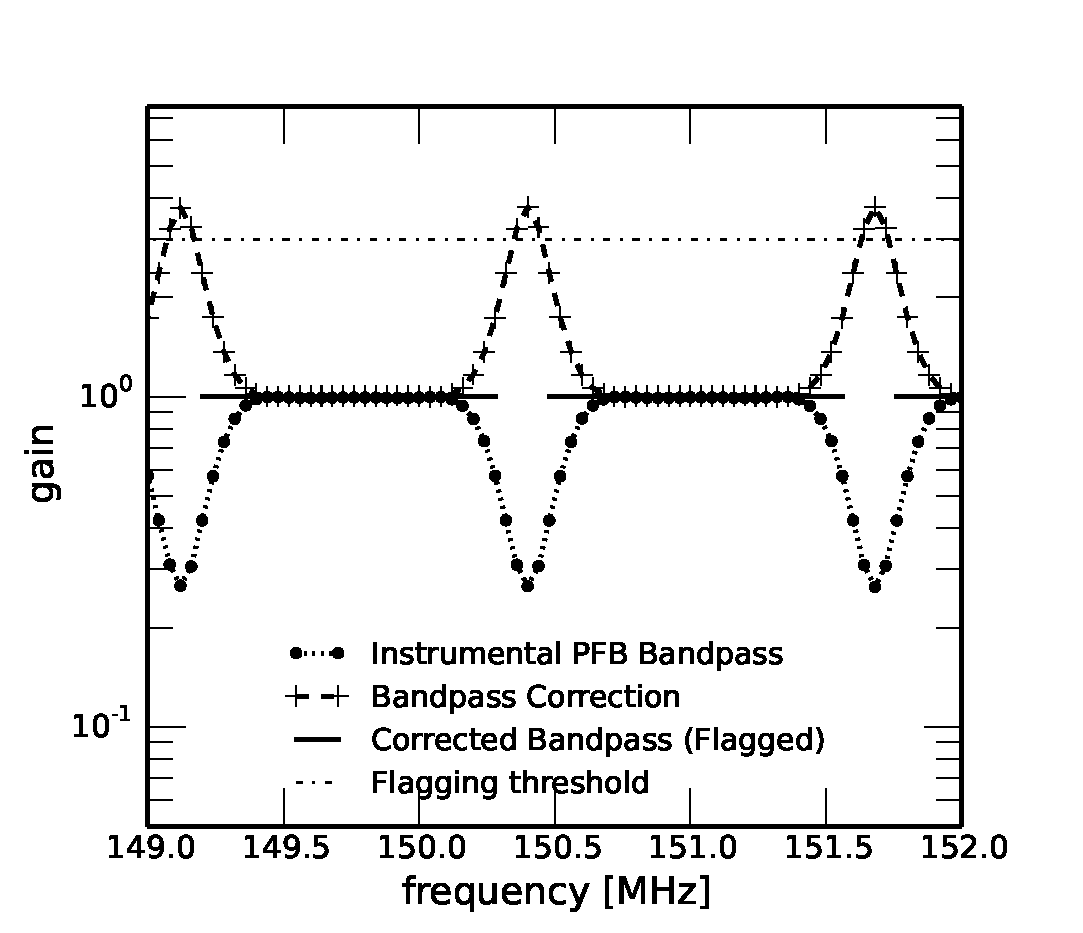
\includegraphics[width=\linewidth]{figures/v1_0/bandpass_properties}
\caption{Bandpass properties used in modeling and analysis of delay spectrum of MWA visibilities. The filled circles joined by dotted lines show the 8--tap PFB bandpass shapes obtained using a Kaiser window with parameter $\beta=5$. The {\it plus} symbols joined by dashed lines are the bandpass correction factors. The solid line shows the flagged (gaps) and gain--corrected bandpass shape, $W_f(f)$. These shapes are repeated every 1.28~MHz for the entire bandwidth of 30.72~MHz centered around 185~MHz. \label{fig:bandpass}}
\end{figure}

Thermal noise in simulated visibilities is estimated assuming a system temperature of $T_\textrm{sys}=90$~K per polarization for all frequency channels for all antenna pairs throughout the course of observation. We take into account the increase in thermal uncertainty in frequency channels that results due to aforementioned bandpass correction. ({\bf Since the bandpass correction is digital, shouldn't the noise stay flat after bandpass correction?})

\subsection{Observation Parameters}\label{sec:obsparms}

The MWA Epoch of reionization targets two primary low-foreground fields. Here we choose to focus on RA = 0h, Dec = -30\arcdeg.   The MWA tracks a patch of sky through antenna beams formed and steered electronically by controlling delay settings of an array of dipoles in a MWA tile. These beamformer delay settings can be changed only in discrete steps. The sky is allowed to drift for a certain period of time (usually $\sim 30$~mins) before the discrete shifts in the beamformer delay settings position the beam to be centered again on the same patch of sky. This process is repeated throughout the course of the observation $\approx 4.86$~hours. Figure~\ref{fig:pointings} illustrates how the apparent pointing oscillates around the desired pointing direction. 

The observations reported here were observed, near the beginning of the campaign, on Aug 23, 2013. This day has been chosen as a reference data set for comparison within the MWA EoR collaboration and was selected on the basis of low number of known system errors from among a long stretch of stable observing.  

Here we have chosen two, 112 second long sections from this night for detailed study.  These were chosen to provide a selection of possible foreground and instrumental conditions.  As an example of ``nominal'' observing setup we choose a zenith pointing; as an example of poor foreground conditions we choose a pointing when the field is 2 hours from zenith.  This pointing has a significantly higher secondary side lobe structure and is recorded when the bright galactic center is well above the horizon. 

The LSTs of these two snapshots are shown in Figure~\ref{fig:pointings} as vertical lines at -1.92~hours (i.e., 22.08~hours) and 0.09~hours which are hereafter denoted as {\it off--zenith} and {\it zenith} pointings respectively. %These pointings (phased array power patterns) are centered at RA = 4\fdg 387, Dec = -29\fdg 86 and RA = -28\fdg 8, Dec = -26\fdg 701, whereas the visibilities themselves are phased to zenith corresponding to RA = -28\fdg 8, Dec = -26\fdg 701, and RA = 1\fdg 35, Dec = -26\fdg 701 respectively.   


\begin{figure}[htb]
\centering
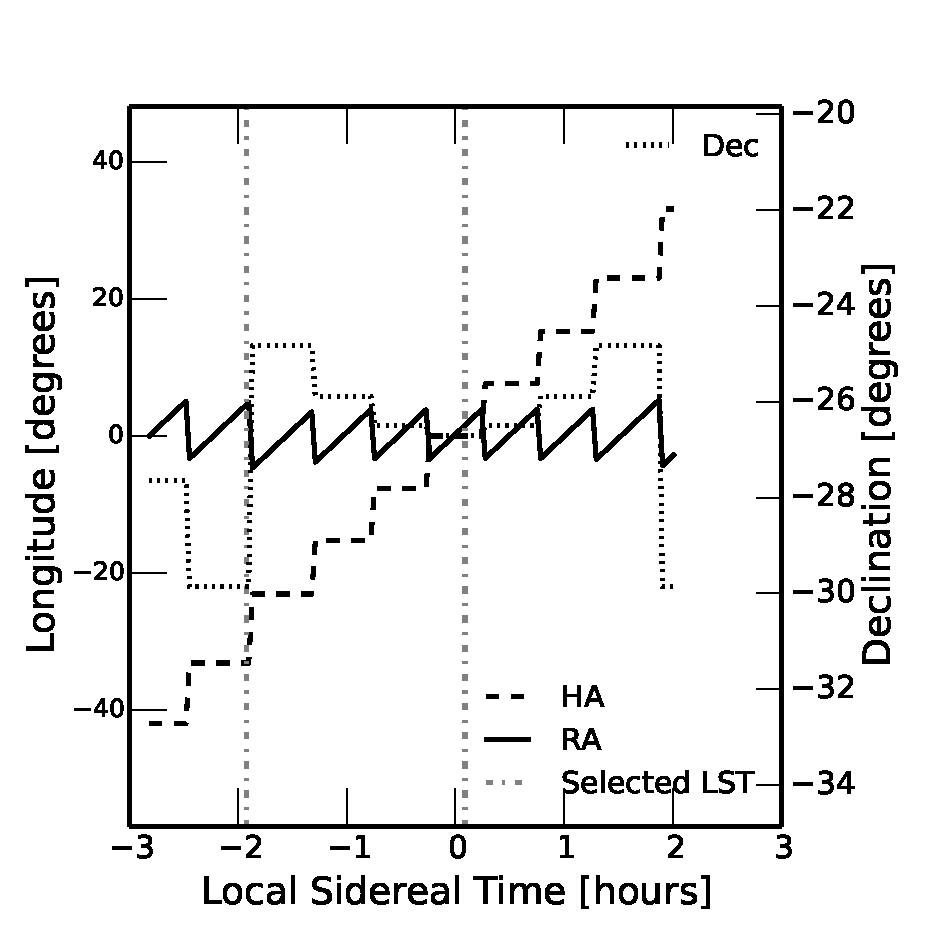
\includegraphics[width=\linewidth]{figures/v1_0/custom_pointings.eps}
\caption{MWA tile beam pointing directions during the course of the observation. The x-axis refers to the Local Sidereal Time (LST) in hours. The axis on the left refers to longitudes, namely, Right Ascension (RA) and Hour Angle (HA) in degrees. Negative values of RA, HA, and LST are to be interpreted as having been wrapped around by 360\arcdeg or 24 hours. The axis on the right refers to the declination of the pointing direction. The RA, HA, and declination are plotted with solid, dashed and dotted line styles respectively. A ``drift and shift'' scheme is used. The sky is allowed to drift for $\sim 30$~mins before the beamformer delay settings change in a discrete step to center the beam around RA = 00h 00m 00.00s, Dec = -30\arcdeg$\,$00\arcmin$\,$00\farcs 0. Dot--dashed vertical lines show the LST of off-zenith and zenith pointings used in our study. \label{fig:pointings}}
\end{figure}

\subsection*{A note on baselines/delay spectra sign convention}

Throughout this paper, $\overline{\mathbf{u}}$ and $\overline{\mathbf{x}}$ are assumed to be on a coordinate system aligned with the local east, north (along local meridian) and upward directions at the MWA site. For the conventions of Fourier transform and its inverse we use in this paper, in accordance with equation~\ref{eqn:delay}, signals from the sky towards east and north are recorded with positive delays on eastward and northward oriented antenna spacings respectively. For instance, at the beginning of the observation, the Galactic center is in the westward sky just about to set. Signals from this direction are recorded with a negative delay on baselines whose antenna spacings are oriented towards the east. Similarly, signals from directions eastward of the local meridian arrive with positive delays on eastward oriented antenna spacings. 

For geometrical intuition, we restrict the orientation ($\theta_b$, measured anti-clockwise from East) of all antenna spacings to lie in the range $-67\fdg 5 \leq \theta_b < 112\fdg 5$. Antenna pairs with spacings oriented in the other half--plane measure conjugate visibilities with delays of equal magnitude but of opposite sign and hence are ignored in our analysis.


\subsubsection{Initial Data processing}\label{sec:data-analysis}
The data are flagged\footnote{\url{http://sourceforge.net/p/aoflagger}} for interference \citep{off12,off10}, removing 3\% of the data and averaged in time  and frequency from the raw 1/2s,40kHz to 2s, 80khz. These data are then calibrated to a simulation of the sky containing 2420 point sources selected from the MWA Commissioning Survey (N.H Walker, in prep).  MWACS was compiled using observations taken with subsets of the array during the final buildout and commissioning. It has a flux limit of 25~mJy and a the declination range of -12\arcdeg to -40\arcdeg evenly covering the field of view of the observations reported here.        The calibration sources are selected to fall within the 5\% primary lobe of the tile beam. The calibration algorithm computes a per channel, per antenna, complex gain solutions averaged to two minute intervals.  The solutions are still fairly low signal to noise so we iteratively project along the antenna and frequency dimensions to capture the relatively independent passband and antenna to antenna variation. First we average the channel gains over all antenna to obtain a high signal to noise measurement of the bandpass.  After applying this single passband, we do a second round of calibration and fit a 2nd order amplitude and first order phase for each antenna. This flattens any residual variation in bandpass and removes small phase slopes due to variation in cable delay. Finally we fit for an additional phase known to be caused by reflection in 150m cables. %possibly could add elaboration, if I knew exactly which version of the cal was done here. doesn't really matter


\subsection{Deconvolution along Delay Axis}\label{sec:CLEAN}

We obtain the delay spectrum of these calibrated visibilities taking the delay transform of each baseline's spectrum (equation~\ref{eqn:delay-transform}) choosing $W'_f(f)$ to be a {\it Blackman--Harris} window function. The spectrum is multiplied by  the additional weight of the flagged channels which occur rarely for interference and at at regular spacing every 1.28~MHz where the edges of coarse channels are known to have a slight aliasing effect.  In delay space, these weights translate into a convolution by a ringing harmonic point spread function (PSF).  We deconvolve this PSF using a one dimensional CLEAN algorithm \citep{tay99} as described for the delay axis by \citet{par09,par12}. The CLEAN procedure iteratively finds and subtracts peak values convolved by the Fourier transform of the weights.   We limit the selection of peaks to modes inside the delay horizon corresponding to smooth spectrum sources on the sky --ie beneath the black line in Figure \ref{fig:fhd_data}.  


\subsection{Delay Spectrum after Delay Deconvolution}\label{sec:data-delay-spectrum}

We show results of delay spectrum from MWA data after deconvolution along delay axis in figure~\ref{fig:fhd_data}. In this plot and others, we plot the amplitude of the delay spectrum sorted by baseline length. Note that no baselines have been averaged together in this plot.  The principle features are the wedge-shaped feature the boundary of which increases approximately linearly with light travel time of the baseline length.  Note that the wedge is not filled out uniformly. Each baseline has a different orientation and resulting response to different sources in the sky. It is this variation that we are investigating.

In these power spectrum units [Mpc$^{-3}$], the reionization power spectrum is expected to be spherically symmetric and decrease quickly with $|k|$.  The brightest signal will occur on the shortest baselines and smallest delays. Thus the region of interest is just above the black horizon line and below the harmonic due to the coarse channels.

 The {\it off--zenith} pointing has emission notably higher than in the {\it zenith} pointing inside the wedge boundaries. This is shown later to be due to response of the array to the bright Galactic center and Galactic plane in the westward sky. Consequently, the contamination into the {\it EoR window} is also higher. Emission in the {\it zenith} pointing is more centrally concentrated due to phasing of power pattern to the zenith, whereas the {\it off--zenith} pointing has a power pattern phased eastward of zenith and is also responsive to emission from angles far away from zenith. 

\begin{figure}[htb]
\centering
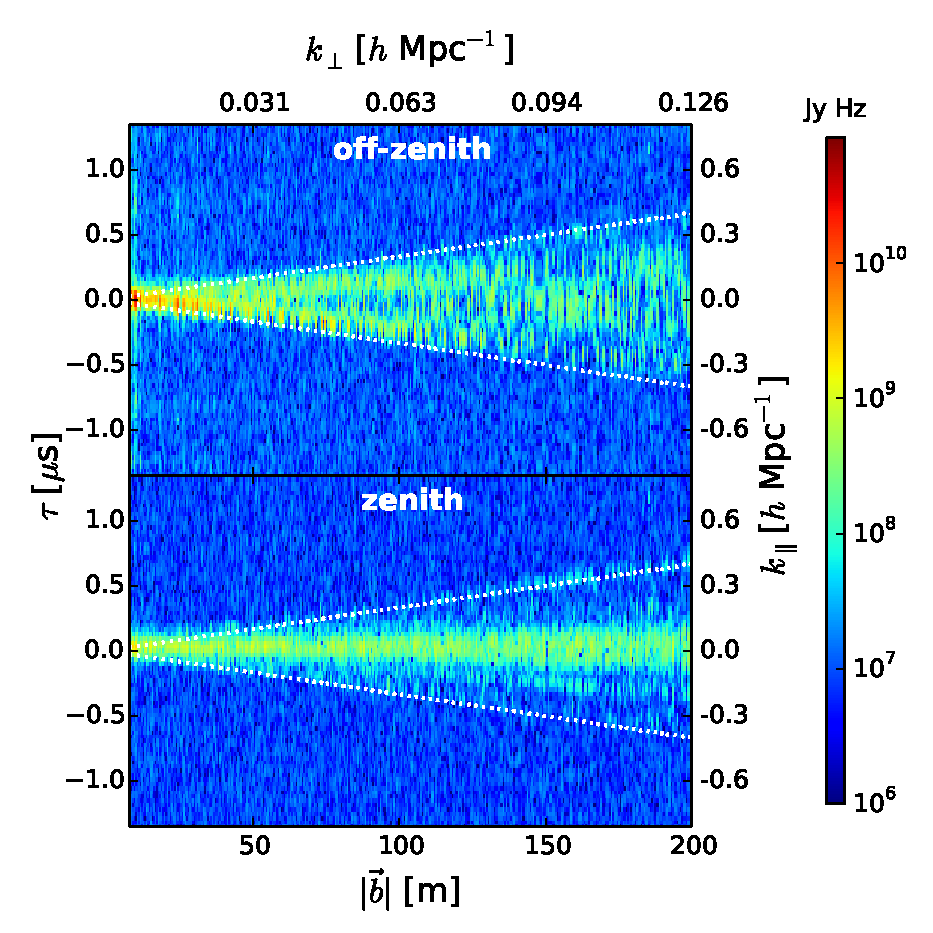
\includegraphics[width=\linewidth]{figures/v1_0/multi_baseline_fhd_delay_spectrum_snapshots.eps}
\caption{ Delay spectrum power spectra of two 112s  Murchison Widefield Array observations of the Epoch of Reionization field at RA=0, Dec=-30.  At top an {\it off--zenith}  pointing when tiles have significant side lobe response in the direction of the galactic center. At bottom a {\it zenith} pointing where side lobes are minimal and the galaxy has completely set.  To get the the power spectrum each baseline is Fourier transformed into delay space ($y$-axis) and the amplitude plotted as a logarithmic color in order of baseline length ($x$-axis). The logarithmic color scale (shown at the right) is common to both panels. White lines mark the boundaries of the {\it foreground wedge} determined by the light travel time across each baseline. Smooth spectrum sources are physically limited to the region below this line.  The various features within the wedge depend on the \emph{orientation} of the baseline, the side lobe structure of the primary beam pointing and the sky at that time. \label{fig:fhd_data}}
\end{figure}

Despite delay deconvolution, we still see leakage beyond the cleaned regions indicating the inability of the deconvolution algorithm to fit the data perfectly. This is predominant at short antenna spacings where the number of delay modes within the horizon. This is because the maximum delay envelope (boundary of the wedge) consists of mixed emission from large portions of the sky into a narrow range of delays and the deconvolution algorithm does not have sufficient support in delay space to fit the delay spectrum. However, we wish to emphasize that the purpose of deconvolution is to rid the delay spectra of instrumental artifacts to the best extent possible in order to see the underlying signatures of foreground emission. It is not our intention in this paper to use the deconvolution as a foreground removal tool. Hence, our discussion and conclusions are valid despite imperfections in deconvolution.

\section{Instrument Modeling}\label{sec:modeling}

We describe power pattern and foreground models we have used in modeling the instrument. %todo

\subsection{Power pattern}\label{sec:power_pattern}

The precise power pattern of the MWA tile ($A(\overline{\mathbf{l}},f)$ in equation~\ref{eqn:obsvis}) is a subject of active investigation. The most precise model currently available is that of Sutinjo et al (2014; submitted?) which models the 4$\times$4 array of bow-tie dipoles as a mutually-coupled array with the overall power-pattern of the dipole modeled via finite element electromagnetic simulation.  To speed simulation we find that a phased array of isotropic radiators at a height of 0.3~m above an infinite ground plane provides a very good approximation to the FEKO simulation. We also assume that each individual dipole signal has random delay fluctuations of rms 0.05~ns, a number in line with the known stability level of the analog signal chain.

\begin{figure}[htb]
\centering
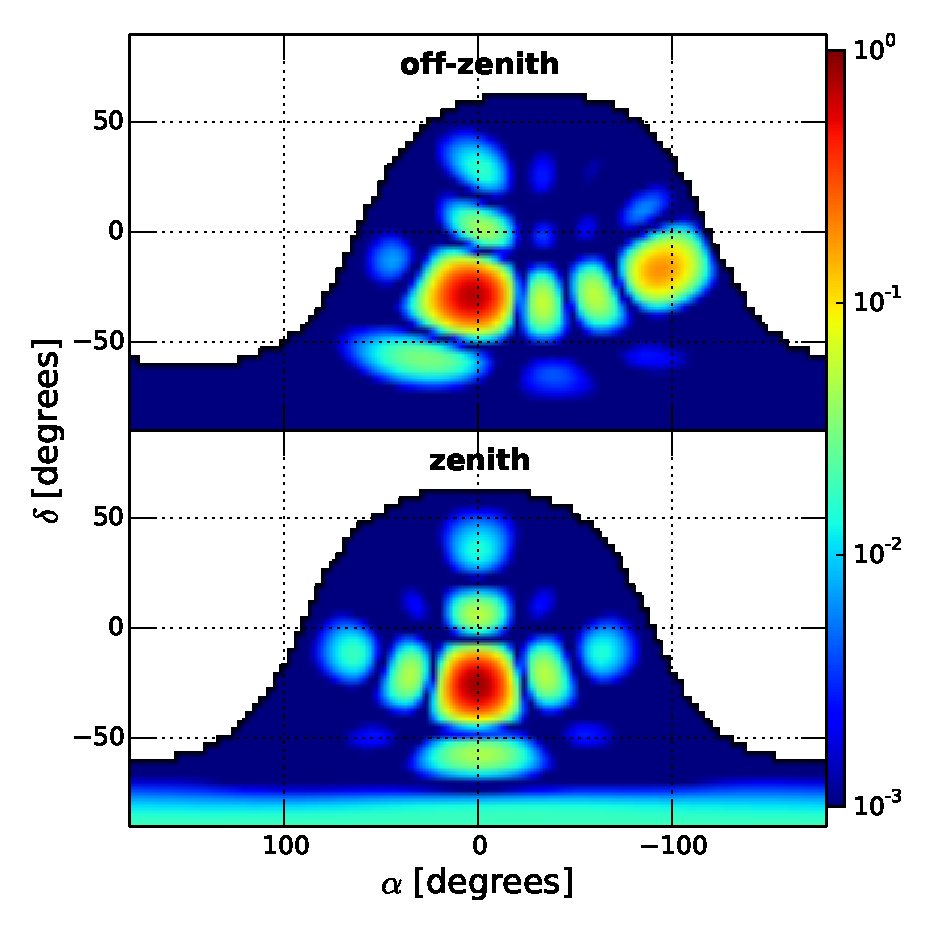
\includegraphics[width=\linewidth]{figures/v1_0/delta_array_powerpattern_0.3m_ground_custom.eps}
\caption{Models of MWA tile power pattern in Right Ascension ($\alpha$) and Declination ($\delta$) coordinates for the off--zenith (top) and zenith pointings (bottom) at 185~MHz. An MWA tile is modeled as a 4$\times$4 array of isotropic radiators placed 0.3~m above the ground plane. Random fluctutations of rms 0.05~ns have been added to delay corrections during the phased addition of voltages from these isotropic radiators. The logarithmic color scale (shown at the right) is common to both panels. \label{fig:power_pattern}}
\end{figure}

\subsection{Foreground Model}\label{sec:foreground}
%todo
The MWA has a very wide field of view ($\gtrsim 20$\arcdeg at 185~MHz) and has non-zero response all the way to the horizon. As we have seen above, foreground sources contaminate the region inside the ``wedge'' with an amplitude that depends on the primary beam amplitude in that direction, with sources at the horizon being closest to the edge of the wedge. 

The degree to which these sources leak power into spectral line of sight modes above the wedge, a region known as the ``EoR Window'', depends primarily on the brightness of foregrounds near the edge of the wedge \citep{thy13,pob13,ved12,par12}. Thus, it is important to consider an all-sky model for foreground objects in evaluating the features seen in the power spectrum instead of restricting to the primary field of view. 

\citet{bea13} estimated the sensitivity of the MWA to EoR H{\sc i} power spectrum detection taking into account thermal noise effects in the {\it Eor window}. \citet{thy13} estimated the sensitivity taking into account the spillover from foreground contamination from unsubtracted extragalactic point sources in the {\t EoR window} besides thermal noise. In this paper, we include the diffuse Galactic emission for enhancing our understanding of foreground signatures in the power spectrum. We use an all-sky foreground emission model that includes both diffuse and bright compact components.  

\subsubsection{Diffuse Foreground Model}\label{sec:DSM}

For the diffuse component, we use an all-sky radio foreground model \citep{deo08} to estimate the emission at 185~MHz. Since this map is predominantly based on the 408~MHz all-sky map of \citet{has82} which has an angular resolution of 0\fdg 85, we smoothed the 185~MHz diffuse emission map to the same resolution. However, to avoid any artifacts from sampling this map, we sample it at $\approx 27$\arcmin~intervals. Using the same model, we use the diffuse emission maps at 170~MHz and 200~MHz to estimate the spectral index map of the diffuse emission model.  

A low resolution version of the diffuse foreground model used is show in figure~\ref{fig:DSM}. Contours of the MWA tile power pattern shown in figure~\ref{fig:power_pattern} are also overlaid. Of notable significance in the {\it off--zenith} pointing is the presence of a portion of the Galactic plane and the bright Galactic center in the visible hemisphere in the westward sky and the MWA tile's power receptivity is significantly high ($\gtrsim 12$\%) in that direction. In the {\it zenith} pointing, the Galactic plane has almost set and the contour level of power pattern in that direction is at least 16 times smaller. 

\begin{figure}[htb]
\centering
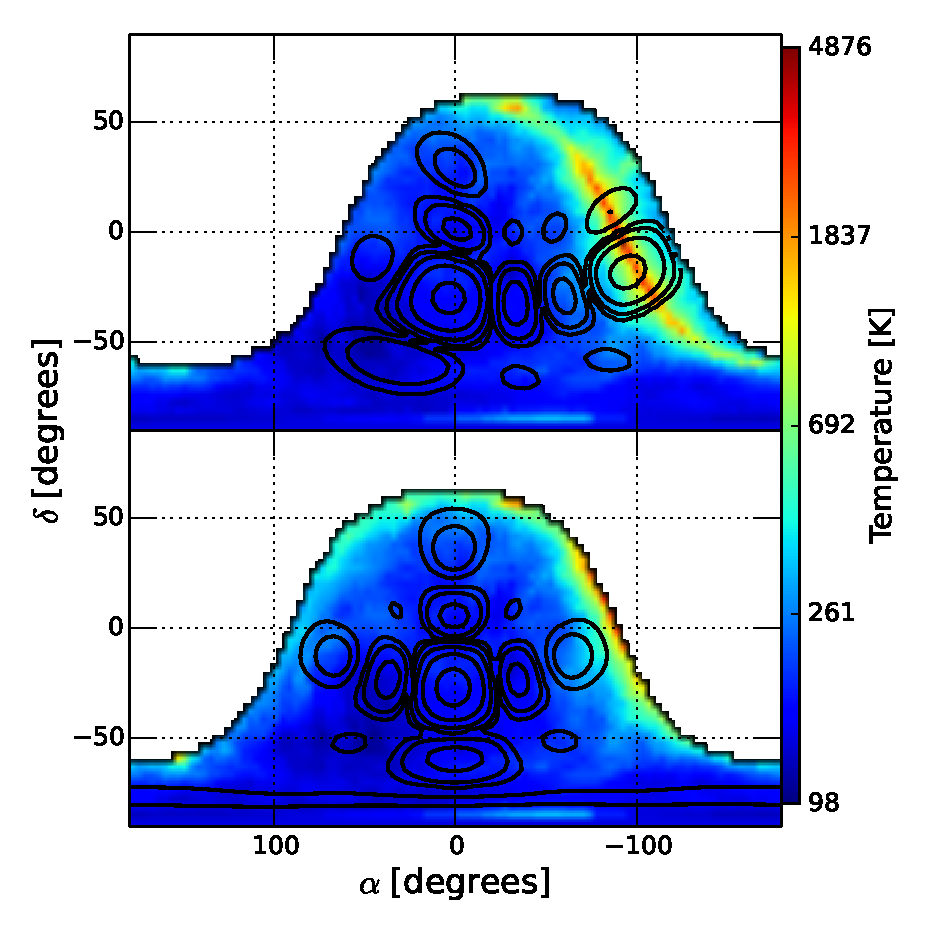
\includegraphics[width=\linewidth]{figures/v1_0/dsm.eps}
\caption{Sky brightness temperature (in K) of the diffuse foreground model at 185~MHz in Right Ascension ($\alpha$) and Declination ($\delta$) coordinates visible during {\it off--zenith} (top) and {\it zenith} (bottom) pointings. The color scale on the right is logarithmic and is common to both panels. Contours of power pattern shown in figure~\ref{fig:power_pattern} are overlaid. The contour levels shown are 0.00195, 0.00781, 0.0312, 0.125, and 0.5. The Galactic center and a portion of the Galactic plane are prominently visible during the {\it off--zenith} pointing and the MWA tile power receptivity is significant ($\gtrsim 12$\%) in that direction. In contrast, emission from the Galactic plane in {\it zenith} pointing is significantly lesser. \label{fig:DSM}}
\end{figure}

\subsubsection{Compact Foreground Model}\label{sec:CSM}

We use a combination of NRAO VLA Sky Survey \citep[NVSS;][]{con98} at 1.4~GHz and Sydney University Molonglo Sky Survey \citep[SUMSS;][]{boc99,mau03} at 843~MHz due to their matched flux sensitivity and angular resolution, and complimentary survey footprints covering the entire sky. The SUMSS catalog covers the sky with declination $\delta < -30$\arcdeg with a limiting peak brightness of 6--10~mJy/beam and an angular resolution of $\sim 45$\arcsec. The NVSS covers the sky with $\delta > -40$\arcdeg with a similar angular resolution and a limiting flux density of $\approx 2.5$~mJy for discrete sources. 

From the SUMSS catalog, we select compact sources whose deconvolved major axes are equal to 0\arcsec. From the NVSS catalog, we excluded objects that overlap with those in the SUMSS survey footprint. Compact sources from NVSS were selected if the convolved major axes were not greater than $\approx 47$\arcsec, which is almost equal to the angular resolution of the survey. Using a mean spectral index of $\langle\alpha_\textrm{sp}\rangle=-0.83$ (flux density, $S(f)\propto f^{\alpha_\textrm{sp}}$) obtained by \citet{mau03} for both NVSS and SUMSS catalog objcts, we calculate the corresponding flux densities at 185~MHz, $S_{185}$. From this subset, we choose compact objects with $S_{185}\geq 10$~Jy. The selection of such bright compact objects is not affected by minor differences in sensitivity of the two surveys. We verified that our selection criteria ensure a similar areal density of sources in the two surveys. 

Based on these criteria, we selected 133 sources from the SUMSS catalog and 336 sources from the NVSS catalog. Together with the diffuse foreground model, we obtain an all-sky foreground model consisting of both compact and diffuse emission.

\begin{figure}[htb]
\centering
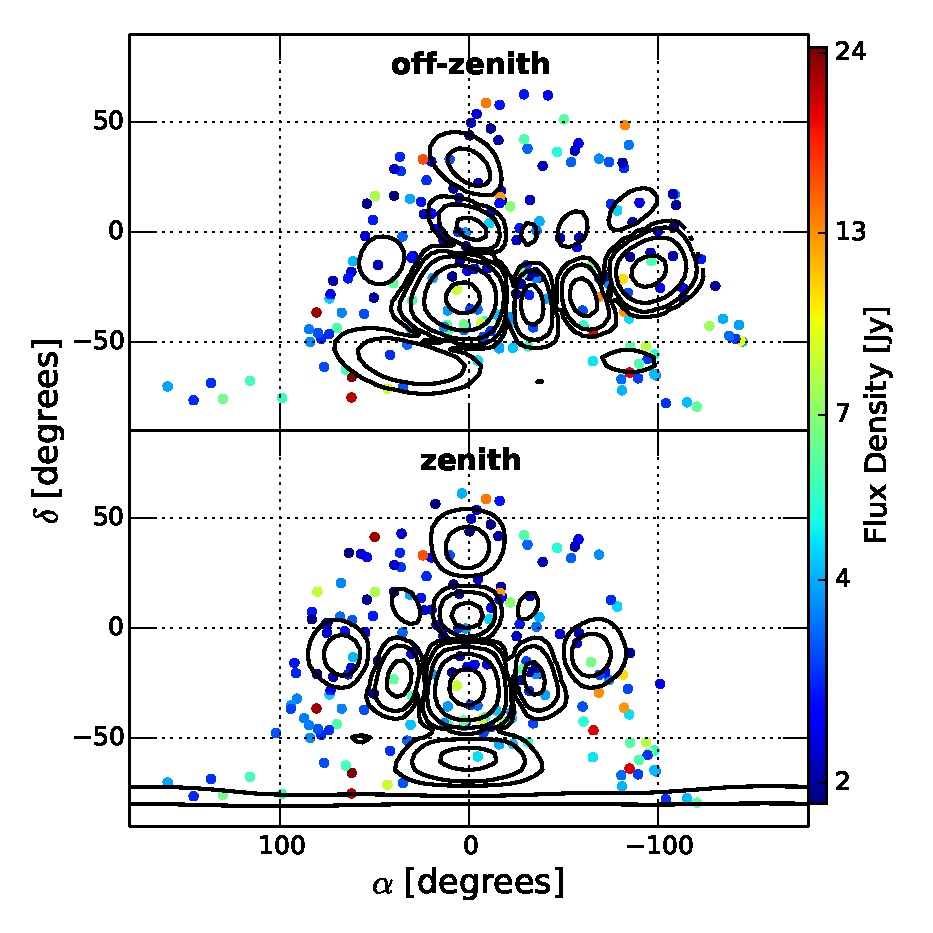
\includegraphics[width=\linewidth]{figures/v1_0/csm.eps}
\caption{Flux densities (in Jy) of bright compact sources at 185~MHz in Right Ascension ($\alpha$) and Declination ($\delta$) coordinates visible during {\it off--zenith} (top) and {\it zenith} (bottom) pointings. The color scale on the right is logarithmic and is common to both panels and corresponds to the color--coded filled circles. Contours of power pattern shown in figure~\ref{fig:power_pattern} are overlaid. The contour levels shown are 0.001953125, 0.0078125, 0.03125, 0.125, and 0.5. The locations of bright compact sources appear to be random.\label{fig:CSM}}
\end{figure}

\subsection{Comparison with Data}\label{sec:data-vs-model}

With the aforementioned all-sky foreground model, and instrumental and observational parameters, we simulate visibilities using equation~\ref{eqn:obsvis}. Figure~\ref{fig:sim_data} shows the amplitude of delay spectrum from {\it off--zenith} and {\it zenith} pointings. Notice the qualitative agreement of amplitude and structure with those obtained from data shown in figure~\ref{fig:fhd_data}. The Galactic center and the Galactic plane visible in the {\it off--zenith} pointing make it appear brighter in the {\it foreground wedge}. 

\begin{figure}[htb]
\centering
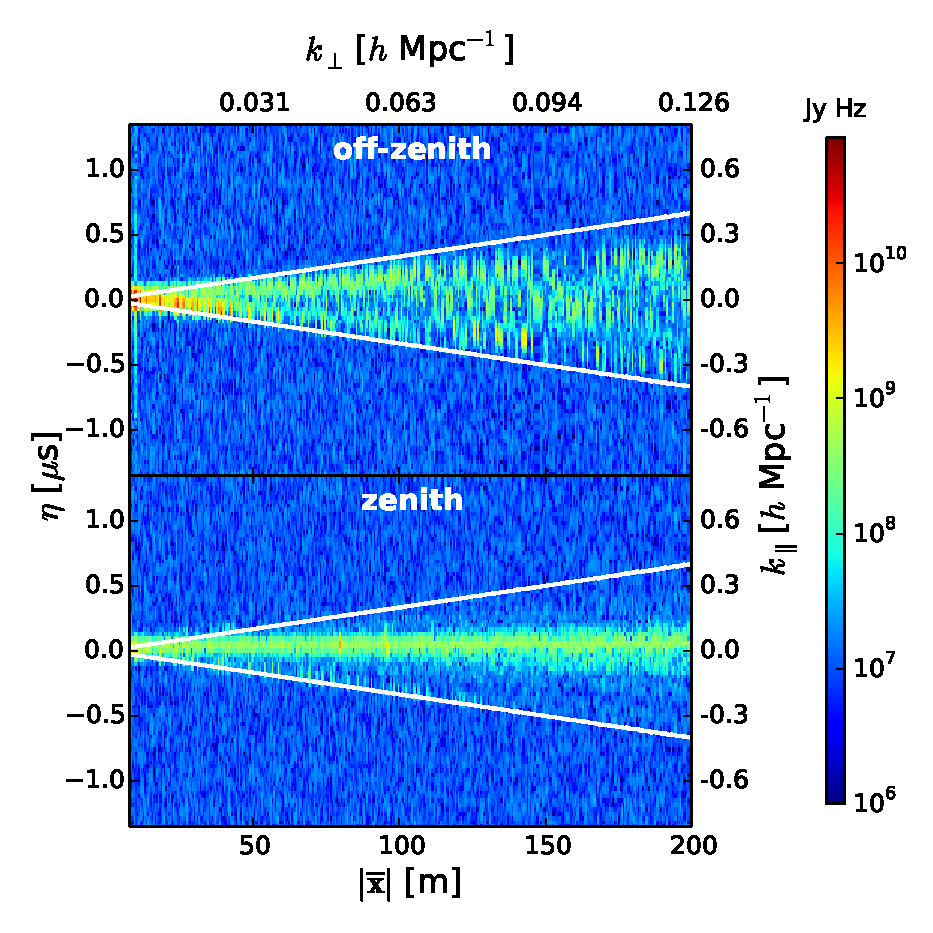
\includegraphics[width=\linewidth]{figures/v1_0/multi_baseline_sim_delay_spectrum_snapshots.eps}
\caption{Delay spectrum amplitude, $|V_\eta(|\overline{\mathbf{x}}|,\eta)|$ (in units of Jy~Hz), obtained with simulations for {\it off--zenith} (top) and {\it zenith} (bottom) pointings. White lines mark the boundaries of {\it foreground wedge} determined by the horizon delay limit and antenna spacing. The features resemble those obtained with MWA data shown in figure~\ref{fig:fhd_data}. The Galactic center and Galactic plane prominently visible in the {\it off--zenith} pointing makes the emission in the {\it foreground wedge} brighter relative to that in the {\it zenith} pointing. The axes and color scale are identical to those in figure~\ref{fig:fhd_data}. \label{fig:sim_data}}
\end{figure}

In order to make a quantitative comparison of delay spectra obtained with the MWA data and our simulations, we consider the following uncertainties. Our foreground models are derived from other higher frequency catalogs and sky maps. The inherent spread in spectral index increases the uncertainty while predicting fluxes at the observed frequency. Using simple error propagation, the fractional error in the delay spectrum caused by the spread in spectral index is $\sim \ln(f_\textrm{orig}/f)\,\Delta\alpha_\textrm{sp}$, where, $f_\textrm{orig}$ is the original frequency at which the catalog or map was created, $f=185$~MHz is the observed frequency, and $\Delta\alpha_\textrm{sp}$ is the spread (HWHM) in spectral index. From \citet{mau03}, we assume $\Delta\alpha_\textrm{sp} \approx 0.35$ for compact sources from NVSS and SUMSS catalogs. Although the model of \citet{deo08} yields a spectral index per direction on the sky, we assume similar uncertainties exist in spectral indices of our diffuse sky model as well, which is predominantly derived from 408~MHz map of \citet{has82}. Thus, fractional errors in delay spectrum from compact foreground objects and diffuse emission are $\sim$70\% and $\sim$30\% respectively. In addition, delay spectra from simulations and data each have uncertainties due to thermal noise with rms, $\Delta V^\textrm{N}_\eta(|\overline{\mathbf{x}}|,\eta) \sim$ 1.4$\times 10^7$~Jy~Hz, where the superscript N stands for thermal noise. We estimate the ratio of delay spectra from data and simulations as, $\rho = |V^\textrm{D}_\eta(|\overline{\mathbf{x}}|,\eta)|\,/\,|V^\textrm{S}_\eta(|\overline{\mathbf{x}}|,\eta)|$, where superscripts D and S denote data and simulation respectively. % Using the aforementioned uncertainties added in quadrature, we estimate the approximate expected uncertainty in $\log_{10}\rho$ and denote it by $\Delta\,\log_{10}\rho$. 

% Figure~\ref{fig:data-sim-ratio} shows the significance of $\log_{10}\rho$ relative to the expected error $\Delta\,\log_{10}\rho$ for all $|\overline{\mathbf{x}}|$ and $\eta$ inside the {\it foreground wedge}. The probability densities and cumulative distributions are shown in black and gray respectively. Also shown are dotted vertical lines which denote equality between $\Delta\,\log_{10}\rho$ and $\log_{10}\rho$. The fraction of the {\it foreground wedge} that lies in between these vertical lines is $\sim$~90\% and $\sim$~95\% for {\it off--zenith} and {\it zenith} pointings respectively. In other words, subject to expected uncertainties, the ratio of delay spectra obtained with MWA data and simulations are consistent with unity at $\sim$~90\% and $\sim$~95\% confidence levels in the {\it off--zenith} and {\it zenith} pointings respectively.

Figure~\ref{fig:data-sim-ratio} shows histograms of the distribution of $\log_{10}\rho$ for the {\it off--zenith} (top panel) and {\it zenith} (bottom panel) pointings respectively inside the {\it foreground wedge}. The median absolute deviation from these distributions correspond to $\sim$~90\% fractional difference between data and modeling on average in either case. This is in line with aforementioned uncertainties in foreground models and thermal noise in measurements. Currently we are significantly limited by unavailability of all--sky foreground models at the observed frequency of 185~MHz. Availability of an accurate foreground model will improve the agreement of simulations with observed data. 

\begin{figure}[htb]
\centering
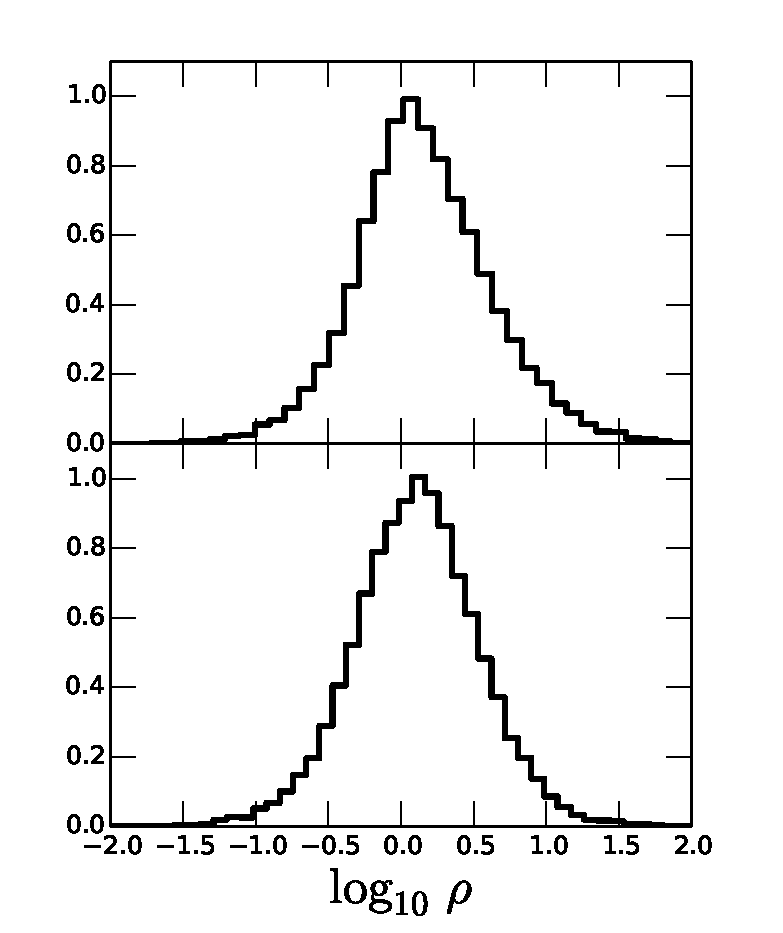
\includegraphics[width=\linewidth]{figures/v1_0/delta_array_histogram_wedge_sim_data_log_ratio_0.3m_ground_custom_gaussian_FG_model_asm_all_sky_nside_64_Tsys_90.0K_185.0_MHz_30.7_MHz_bnw2.0.eps}
\caption{Histogram of logarithm of ratio of observed to simulated visibilities restricted to the {\it foreground wedge} --i.e. within the white lines of Figure \ref{fig:sim_data}-- for the {\it off--zenith} (top) and {\it zenith} (bottom) pointings. Median absolute deviations of $\log_{10}\rho$ are 0.29 and 0.27 respectively. A value of zero indicates when the ratio $\rho=1$. \label{fig:data-sim-ratio}}
% 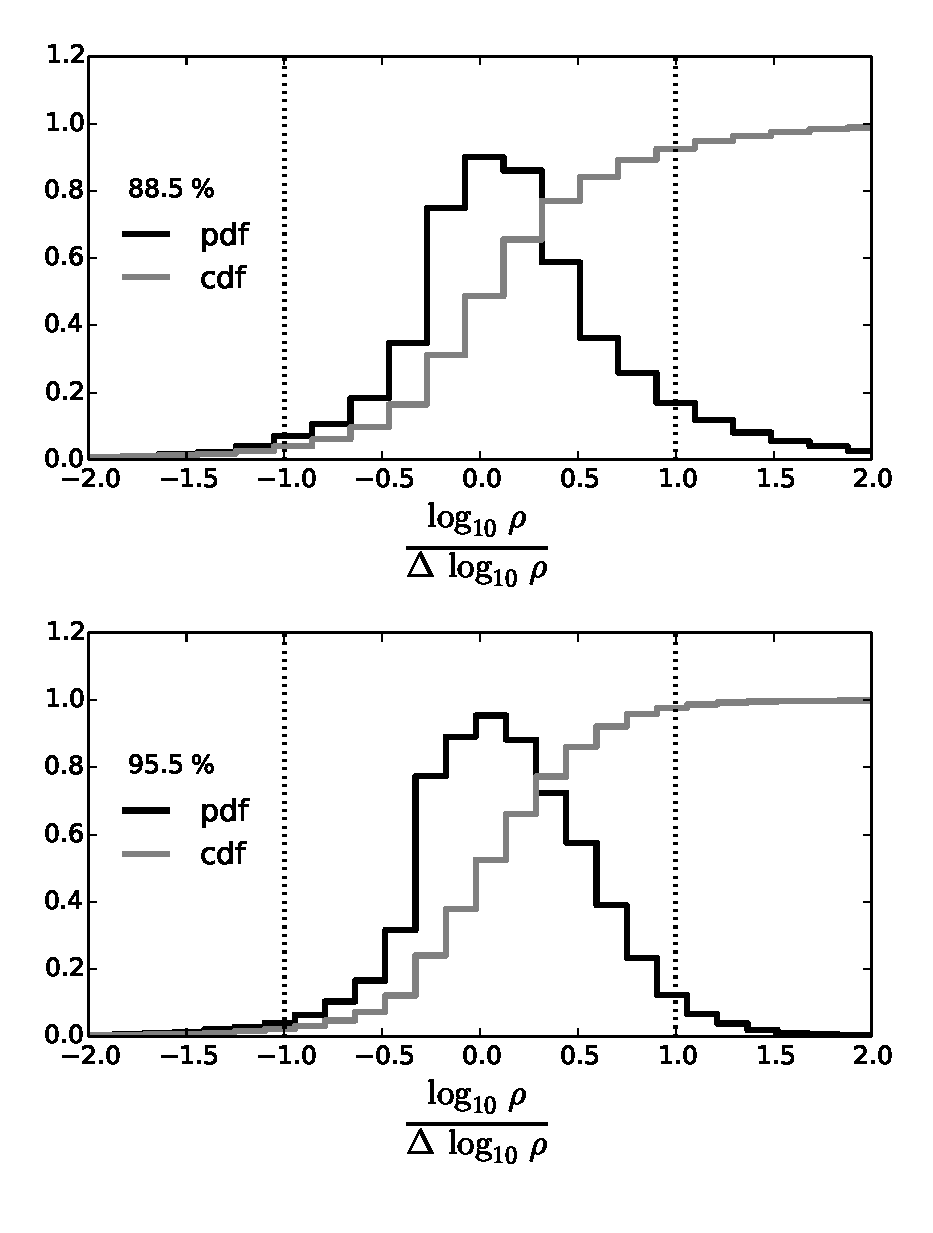
\includegraphics[width=\linewidth]{figures/v1_0/delta_array_histogram_wedge_sim_data_snr_log_ratio_0.3m_ground_custom_gaussian_FG_model_asm_all_sky_nside_64_Tsys_90.0K_185.0_MHz_30.7_MHz_bnw2.0.eps}
% \caption{Significance of logarithm of ratio of observed to simulated visibilities relative to expected uncertainty restricted to the {\it foreground wedge} for the {\it off--zenith} (top) and {\it zenith} (bottom) pointings. Probability densities and cumulative distributions are shown in black and gray respectively. Region inside the dotted vertical lines denotes when the ratio, $\rho$, is consistent with unity subject to expected uncertainty. Also indicated in percentages are confidence levels estimated conservatively for such a consistency. They are $\sim$~90\% and $\sim$~95\% for {\it off--zenith} and {\it zenith} pointings respectively. \label{fig:data-sim-ratio-snr}}
\end{figure}

These uncertainties are presented only to confirm the qualitative agreement already seen between figures~\ref{fig:fhd_data} and \ref{fig:sim_data} and are not intended to serve as a comprehensive estimate of all uncertainties involved. However, since we have not accounted for numerous other uncertainties, especially in the data, such as uncertainties in the antenna power pattern, calibration, radio frequency interference (RFI), and wide field imaging effects, our estimates are conservative. Accounting for such uncertainties will only improve our confidence level in this comparison. Our primary objective is to explore in detail the foreground signatures embedded in the {\it foreground wedge}.

\section{Delay Spectrum Analysis}\label{sec:delay-spectrum-analysis}

Having established that the model, by and large, matches the data, we proceed to examine in further detail the signatures seen in the modeled delay spectra. 

A number of factors are responsible for the characteristics noted in the delay spectra obtained from data and through modeling. We address these factors below:
\begin{itemize}

\item {\it Sky Model}: Our model of the sky consists of bright compact sources and diffuse emission on diverse spatial scales as seen from figures~\ref{fig:DSM} and \ref{fig:CSM}. It also consists of localized regions of strong emission such as the Galactic plane and Galactic center. The resulting sky emission is anisotropic. In fact, the patch of sky for MWA observations is chosen from regions of low foreground emission. In our detailed study, we have divided the transiting sky into four different ``bow-tie'' shaped regions with equal areas around zenith as the origin. This results in the ability to attribute the features in the delay spectrum to eight different sectors of the sky. %TODO possibly reference sections or figures here?

\item {\it Antenna Pair Orientation}: Since the spatial structure of our foreground model is not expected to be isotropic, we divide our antenna pairs by their orientation ($\theta_\textrm{b}$) measured counter-clockwise from East. We use the following bins: $-67\fdg 5\le \theta_\textrm{b} < -22\fdg 5$, $-22\fdg 5\le \theta_\textrm{b} < 22\fdg 5$, $22\fdg 5\le \theta_\textrm{b} < 67\fdg 5$, and $67\fdg 5\le \theta_\textrm{b} < 112\fdg 5$. The bin centers are oriented towards South-East, East, North-East, and North respectively. Since delays depend on antenna pair orientation, binning by orientation allows us to match delay spectrum features to different sky directions.

\item {\it Tile Pointing and Power Pattern}: Since the MWA tiles are steered electronically, the power pattern of the tile changes in any observing mode that tracks the source. The pointing system is capable of steering to points on a regular $\sim$7\arcdeg grid.  During observations we allow the sky to drift across the nearest available pointing, shifting between grid points as necessary. In our study, we take into account the effect of changing power pattern of the antennas on the delay spectrum (Figure~\ref{fig:power_pattern}). The LST of our data ranges from $\sim$~21 hours through $\sim$~2 hours, and for our analysis we chose {\it off--zenith} and {\it zenith} pointings shown in figure~\ref{fig:pointings}. 

\item {\it Instrumental Passband}: The instrumental passband characteristics have a direct effect on the delay transform owing to the Fourier relationship between the two. Due to excision of noisy and aliased edge channels repeated in each coarse channel of our passband, we saw repeated patterns of the {\it foreground wedge} in the delay spectra. As already mentioned earlier, we have used the deconvolution algorithm ({\it CLEAN}) to rid the delay spectra of band shape effects. Since this paper focuses on studying the effects of foreground on the delay spectra, we do not pursue the characterization of artifacts from the band shape and imperfections in {\it CLEAN} deconvolution.

\end{itemize}

%The foreground signatures we henceforth identify in the delay spectrum are characterized as arising out of the aforementioned factors. Due to numerous combinations of such factors, we use unique annotations to characterize these signatures.   

It may be noted that numerous features overlap at varying levels of significance depending on the combinations of parameters. We assign the features to their predominant causes. Secondly, we have used noiseless cases to clearly illustrate the observed foreground signatures. With the addition of noise in the visibilities which is subject to observing time, some of the weaker features may not be as prominently visible. Since the foreground signatures are far too numerous and they reside in a vast volume of parameter space such as antenna pair orientation, power pattern, patch of sky under observation, and instrumental configuration, we highlight only some examples of the most notable features observed in the delay spectrum of foreground emission.

\subsection{Diffuse Foreground: Input model}\label{sec:diffuse}

Figure~\ref{fig:noiseless-dsm-delay-spectrum} shows the amplitude of delay spectrum, $|V_\eta(|\overline{\mathbf{x}}|,\eta)|$, simulated with the diffuse foreground model. The top and bottom panels correspond to {\it off--zenith} and {\it zenith} pointings respectively. 

\begin{figure}[htb]
\centering
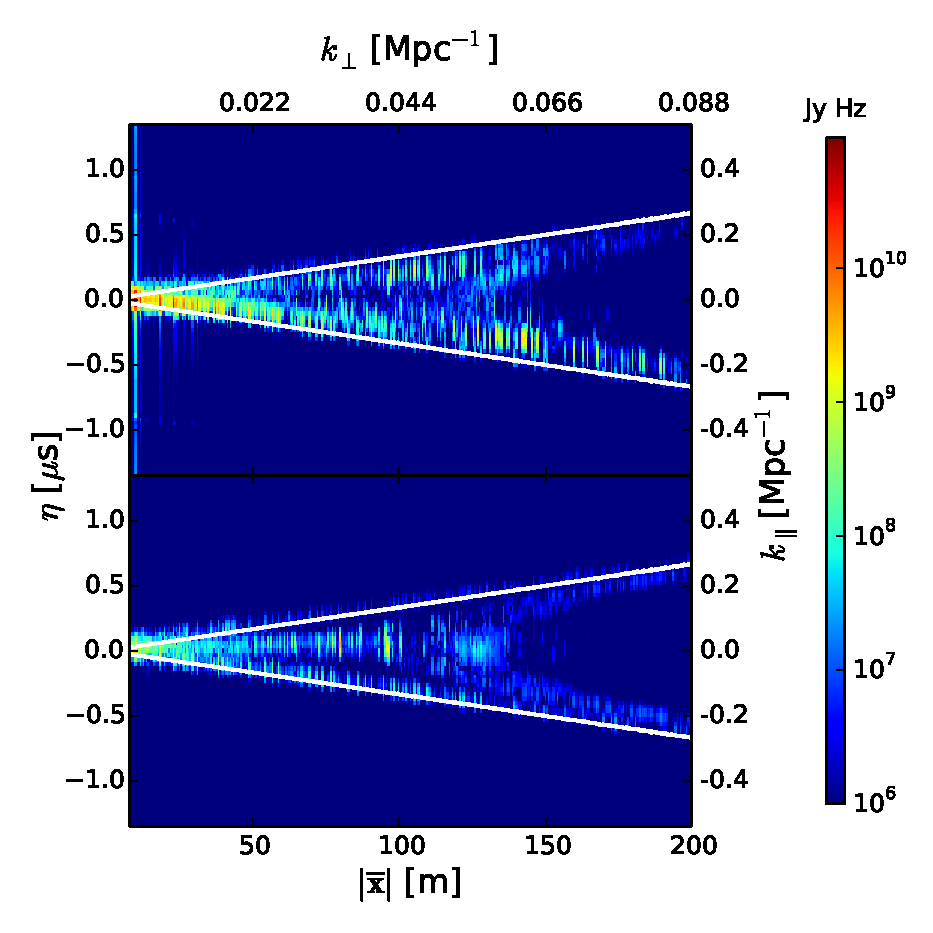
\includegraphics[width=\linewidth]{figures/v1_0/delta_array_multi_baseline_CLEAN_noiseless_visibilities_0.3m_ground_custom_gaussian_FG_model_dsm_all_sky_nside_64_Tsys_90.0K_185.0_MHz_30.7_MHz_bnw2.0.eps}
\caption{Delay spectrum amplitude, $|V_\eta(|\overline{\mathbf{x}}|,\eta)|$ (in units of Jy~Hz), obtained with simulations for {\it off--zenith} (top) and {\it zenith} (bottom) pointings for the diffuse foreground model without any thermal noise. White lines mark the boundaries of {\it foreground wedge} determined by the horizon delay limit and antenna spacing. The logarithmic color scale is common to both panels. In the {\it zenith} pointing, diffuse emission delay spectrum has a {\it two--pronged fork}--shaped structure and is present even at wide antenna spacings. \label{fig:noiseless-dsm-delay-spectrum}}
\end{figure}

Here we examine in detail some examples of interesting features observed with the diffuse foreground model.

\subsubsection{Galactic Center on Eastward Antenna Spacings}\label{sec:GC-east}

The most prominent signature seen in the {\it off--zenith} pointing (top panel of figure~\ref{fig:noiseless-dsm-delay-spectrum}) is due to the bright Galactic center situated on the far west on one of the sidelobes of the power pattern. It appears as a bright branch in the delay spectrum near the negative delay horizon delay limit. This feature is strongest at short antenna spacings and fades with increase in antenna spacing. This Galactic center signature is almost invisible in the {\it zenith} pointing because the Galactic center has already set over the horizon (see bottom panel in figure~\ref{fig:noiseless-dsm-delay-spectrum}). 

\subsubsection{Diffuse Emission Power Spectra}\label{sec:diffuse-features}

As we also see in Figure~\ref{fig:noiseless-dsm-delay-spectrum}, diffuse emission from within the field of view manifests in the {\it off--zenith} pointing as a branch at the top of the wedge, while in the {\it zenith} pointing it shows up at near zero delay. The former is seen at positive delays because the main lobe of the power pattern is centered eastward of zenith, whereas in the latter it is centered at zenith. As we see from Equation \ref{eqn:obsvis}, each baseline measures a single spatial mode on the sky with an angular size scale inverseley proportional to length of the baseline projected in the direction of emission.  Thus, on the {\it zenith} pointing, the signature of the smooth sky model, the horizontal line at zero delay, fades away on antenna spacings wider than $\gtrsim 125$~m because the sky model is devoid of spatial structures on scales $\lesssim$~0\fdg 75. On the off-zenith pointing we see power out to much longer baselines.

\subsubsection{Diffuse Emission on Wide Antenna Spacings}\label{sec:diffuse-long-baselines}

A very interesting signature of diffuse emission is revealed at regions near the positive horizon delay limit in the {\it off--zenith} pointing and at both positive and negative horizon delay limits in the {\it zenith} pointing even on wide antenna spacings (125~m~$\lesssim \overline{\mathbf{x}}\le$~200~m) contrary to expectations, which are not expected to be sensitive to diffuse emission. We claim this is because wide antenna spacings appear shortened due to projection effects when sensitivity towards off--axis emission, especially towards the horizon, is concerned. It naturally holds for short antenna spacings as well. Thus, diffuse emission from far off--axis directions manifests as an edge--heavy {\it two--pronged fork} across all antenna spacings. It decreases in strength with increasing antenna spacing as expected but is present in all orientations of the antenna spacing vector. This contributes to a {\it pitchfork}--shaped feature which will be discussed later in \S\ref{sec:pitchfork} in more detail.

\subsection{Compact Foregrounds}\label{sec:compact}

Figure~\ref{fig:noiseless-csm-delay-spectrum} shows the delay spectrum compact source sky model for {\it off--zenith} and {\it zenith} pointings (shown in Figure~\ref{fig:CSM}) in the top and bottom panels respectively. 

\begin{figure}[htb]
\centering
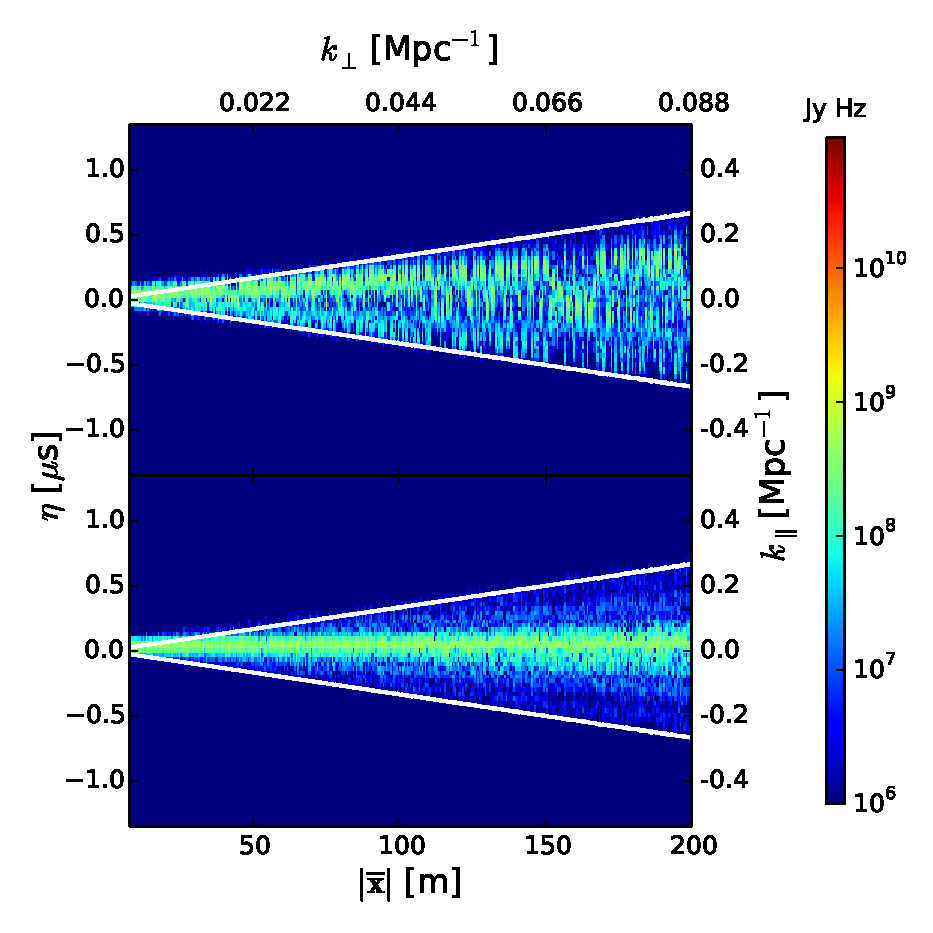
\includegraphics[width=\linewidth]{figures/v1_0/delta_array_multi_baseline_CLEAN_noiseless_visibilities_0.3m_ground_custom_gaussian_FG_model_csm_all_sky_nside_64_Tsys_90.0K_185.0_MHz_30.7_MHz_bnw2.0.eps}
\caption{Delay spectrum amplitude, $|V_\eta(|\overline{\mathbf{x}}|,\eta)|$ (in units of Jy~Hz), obtained with simulations for {\it off--zenith} (top) and {\it zenith} (bottom) pointings for the compact objects foreground model without any thermal noise. White lines mark the boundaries of {\it foreground wedge} determined by the horizon delay limit and antenna spacing. The logarithmic color scale is identical to that in Figure~\ref{fig:noiseless-dsm-delay-spectrum}. Emission from compact objects gives rise to centrally concentrated features in the {\it foreground wedge}.\label{fig:noiseless-csm-delay-spectrum}}
\end{figure}

In contrast to delay spectrum of diffuse emission, compact emission manifests as a center--heavy structure in the delay spectrum with either pointing. This contributes to the {\it pitchfork} feature which will be discussed in detail in \S\ref{sec:pitchfork}. Below we summarize some specific notable features obtained with our compact objects foreground model.

\subsubsection{Compact Emission in Power Pattern Main Lobe}\label{sec:csm-main-lobe}
The response of an interferometer to a compact source is, to first order, flat with respect to baseline length. Therefor the distribution of sources within the primary field of view depends mainly on how the beam pattern maps to delay space for each antenna pair. Since the main lobe of the power pattern in the {\it off--zenith} pointing is centered eastward of zenith, the bulk of the compact foreground emission is seen in a branch with positive delay corresponding to the position of the pointing center. In the {\it zenith} pointing compact emission from the same patch of sky is seen as a bright horizontal arm at zero delay  since the main lobe of the power pattern is centered at zenith. 

\subsubsection{Compact Emission in Power Pattern Sidelobes}\label{sec:csm-side-lobe}

Foreground emission in zero delay and negative delay regions in the {\it off--zenith} pointing is caused by compact objects co--located with sidelobes of the power pattern. On the other hand, compact objects co--located with sidelobes of power pattern in the {\it zenith} pointing are revealed as distinct but faint branches at positive and negative delays depending on the orientation of antenna spacing and direction of emission on the sky. 

\subsection{Combined Foreground Model}\label{sec:composite}

Delay spectra from the all-sky foreground model in our study display a composite feature set drawn from the features of compact and diffuse foreground models. Here we compare the relative strengths of emission from different spatial scales in our all--sky composite foreground model. 

\subsubsection{{\it Pitchfork} Effect}\label{sec:pitchfork}

When not dominated by the bright emission from the Galactic center, which happens only for certain pointings at certain times, the delay spectrum of the combined foreground model is dominated, in somewhat equal measure, by diffuse and compact emission. This is illustrated by a more detailed examination of the {\it zenith} pointing in our study. 

Figure~\ref{fig:pitchfork-baselines} shows delay spectra of three antenna pairs of different antenna spacings oriented northward during the {\it zenith} pointing; each is a different vertical slice of the two dimensional power spectrum plots shown in Figures \ref{fig:fhd_data} et al. The diffuse, compact, and composite components are are shown as dotted, dashed, and solid lines respectively. The horizon delay limits are shown as vertical dot--dashed lines. The gray shaded area denotes the envelope of expected uncertainty in the delay spectrum. Sources inside the {\it foreground} wedge (between the horizon delay limits) are dominated by the $\sim$70\% error in predicting the spectral index of compact foreground objects, outside the wedge thermal noise dominates. 

\begin{figure}[htb]
\centering
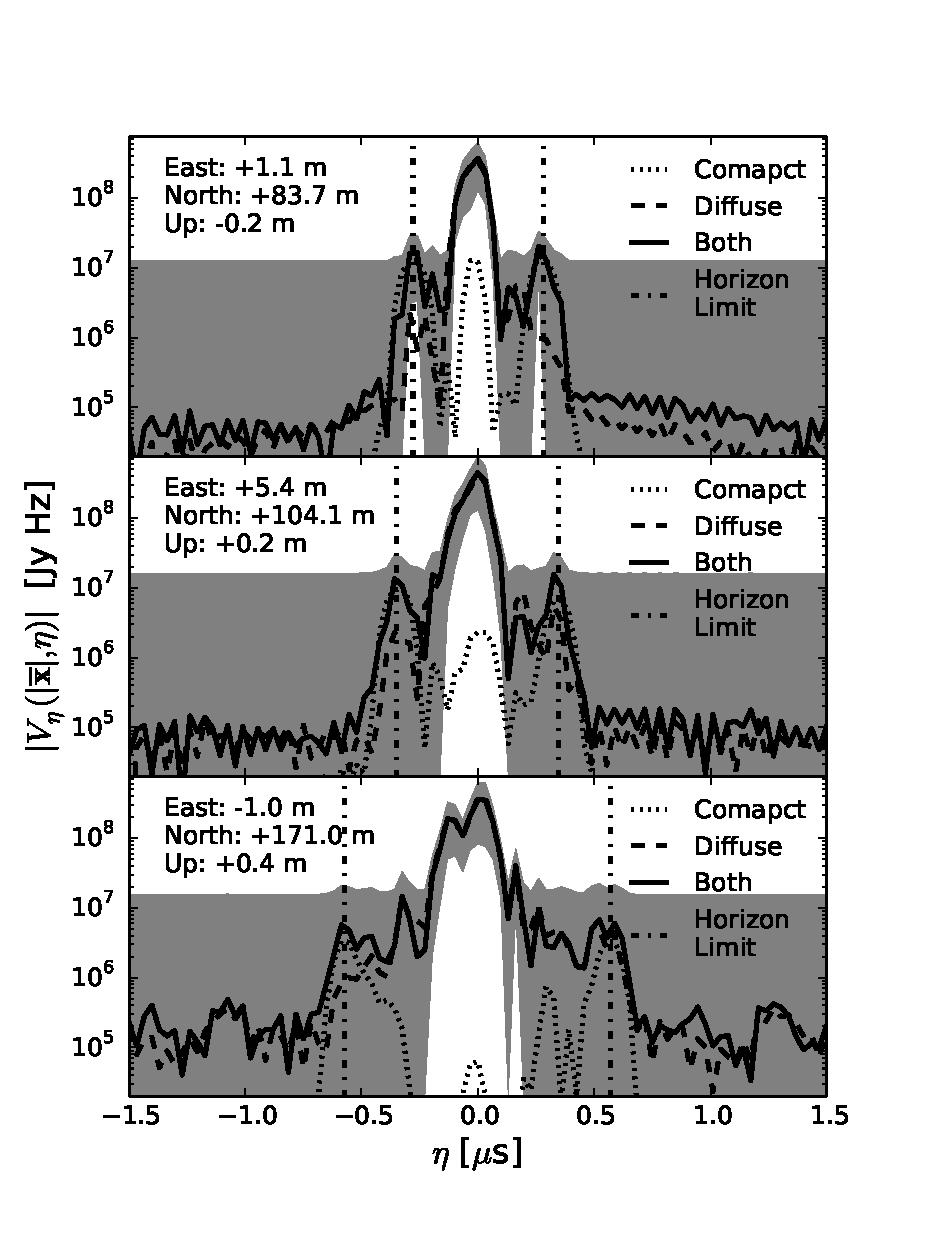
\includegraphics[width=\linewidth]{figures/v1_0/delta_array_3_baseline_comparison_visibilities_0.3m_ground_custom_gaussian_FG_model_csm_all_sky_nside_64_Tsys_90.0K_185.0_MHz_30.7_MHz_bnw2.0.eps}
\caption{Absolute value of delay spectrum, $|V_\eta(\overline{\mathbf{x}},\eta)|$, for three chosen antenna spacings of length: $\sim$84~m ({\it top}), $\sim$105~m ({\it middle}), and $\sim$170~m ({\it bottom}). The antenna spacing vector is specified in each panel along East, North and Upward directions. The dotted, dashed and solid lines denote contributions from diffuse emission, compact objects and composite foreground model respectively. The dot--dashed lines mark the horizon delay limits. The shaded region denotes the envelope of uncertainty around expected values for composite model. This uncertainty is dictated by uncertainties in spectral indices of foreground models inside the delay horizon delay limits. Outside the horizon delay limits, it is predominantly due to thermal noise. Compact objects dominate the central regions of power spectrum while both components, especially diffuse emission on short antenna spacings, dominate near the horizon delay limits, giving rise to a {\it pitchfork}--shaped structure. \label{fig:pitchfork-baselines}}
\end{figure}

The zero--delay peak (corresponding to the main lobe in the power pattern) with a value of $\sim 10^8$--$10^9$~Jy~Hz, independent of antenna spacing, is predominantly determined by compact foreground objects. The corresponding peak at zero--delay from diffuse foreground model is at least 10 times fainter and decreases drastically with increase in antenna spacing. This is the response expected from different antenna spacings towards compact and diffuse foreground objects. 

Near the horizon delay limits at shorter antenna spacing, diffuse emission is brighter than that from compact objects.  Diffuse emission does not decrease as rapidly with increasing antenna spacing as was seen at zero--delay. In fact, even on widely spaced antennas, {\emph diffuse emission in the delay spectrum near the horizon delay limits exceeds that in the main lobe by more than two orders of magnitude}. This is due to apparent shortening of antenna spacings projected in the direction of smooth emission entering far from the primary field of view. This demonstrates the edge--heavy {\it two--pronged fork} feature discussed in \S\ref{sec:diffuse-long-baselines}.

The resulting baseline dependent power spectrum from a composite foreground model that combines diffuse and compact object emission consists of center--heavy features on all antenna spacings from compact objects and edge--heavy features from both components especially diffuse emission even on wide antenna spacings. Henceforth, we call this as the {\it pitchfork} structure in the {\it foreground} wedge.

All these observations are consistent with those from Figures~\ref{fig:noiseless-dsm-delay-spectrum} and \ref{fig:noiseless-csm-delay-spectrum}. The observability of the predicted {\it pitchfork} signature depends on the relative levels of uncertainty in the foreground model and thermal noise. In our simulations, since thermal noise in these very short snapshots is $\gtrsim 10^7$~Jy~Hz, and features near the horizon delay limits are $\sim 10^7$~Jy~Hz, the {\it pitchfork} feature is not expected to be detected in a noisy scenario although this feature is marginally visible in the {\it zenith} pointing of the observed data (see Figure~\ref{fig:fhd_data}). We attribute this to differences between our foreground model and the actual sky. However, with improvements to the foreground model and the addition of more data to reduce the thermal noise, we are confident the {\it pitchfork} signature in delay spectrum will be observed with high significance.

We also note that increasing the antenna spacing results in progressively improving the resolution along delay axis by increasing the number of delay bins inside the {\it foreground wedge}. This improves the localization of foreground objects whose signatures are imprinted in the delay spectrum. For instance, there is an increase in the number of secondary peaks in the delay spectrum between zero--delay and horizon delay limits as antenna spacing increases from $\sim$84~m to $\sim$170~m. In this case, these correspond to sidelobes of the power pattern that lie between the main lobe and the horizon along the North--South direction. In short antenna spacings, due to relatively lower resolution along delay axis inside the {\it foreground wedge} and a consequent loss of localization of direction of foreground emission, these secondary peaks blend in with other major peaks and are not distinctly visible. These findings are consistent with the discussion in \S\ref{sec:csm-side-lobe}.

In summary, the brightest signature ($\gtrsim 10^{10}$~Jy~Hz) is that of the Galactic center in the {\it off--zenith} pointing co--located at a westward sidelobe with a significantly high gain. The next brightest signature ($\sim 10^8$--$\sim 10^9$~Jy~Hz) is caused by compact emission appearing to be concentrated in the inner regions of the foreground wedge (near zero delays) rather than towards the edges. Diffuse emission co--located at the main lobe of the power pattern is fainter by approximately an order of magnitude relative to compact emission from the same region for a $\sim 84$~m antenna spacing but unlike the latter, diffuse emission decreases rapidly by over two orders of magnitude as antenna spacing is widened to $\sim 170$~m. However, diffuse emission is significantly high near horizon delay limits compared to main lobe of the power pattern as antenna spacing is widened. This leads to edge--heavy features in the delay spectrum. Complemented by the center-heavy compact foreground features, we have demonstrated the presence of a {\it three--pronged pitchfork}--shaped signature in the delay spectrum of foreground sky.

\section{Screening of Severe Foreground Contaminated Interferometers}\label{sec:fg-grading}

The delay spectrum, $V_\eta(\overline{\mathbf{x}},\eta)$, not only carries information on spatial scales of foreground emission but also offers a unique advantage of viewing the sky through a combination of antenna spacing vector and the delay axis. This allows us to programmatically screen data for antenna spacings that are severely contaminated by foregrounds which can be weighted appropriately during data analysis. While the {\it foreground wedge} is a region of high foreground contamination, of particular interest to the EoR community is foreground contamination near horizon delay limits. These regions are responsible for significant spillover into the relatively clean {\it EoR window} due to spectral response of the instrument and foregrounds. 

With a foreground model known {\it a priori} in which locations of very bright foreground objects such as the Galactic center or AGN are available, we can predict their response across antenna spacings as a function of observing parameters such as LST, power pattern, etc. Specifically, we can pick antenna pairs where these bright foreground objects will be visible at delays near horizon delay limits. One such example is already provided in our study. The Galactic center is the most dominant source of foreground contamination in the {\it off--zenith} pointing. Since it is located in the western sky, it is most distinctly seen near the negative horizon delay limit on eastward oriented antenna spacings in the delay spectrum (see Figures~\ref{fig:fhd_data}, \ref{fig:sim_data} and \ref{fig:noiseless-dsm-delay-spectrum}, and \S\ref{sec:GC-east}). In fact these figures illustrate quite well the leakage beyond the {\it foreground wedge} into the {\it EoR window} due to these extremely bright sources near the edge of the wedge. In practice, we could downweight these antenna spacings for the specific LST to mitigate the effects of spillover from such foreground contamination in EoR studies. With spatial scales of such objects known, besides downweighting based on antenna spacing orientation, we could also downweight based on antenna spacing distance. For instance, a bright compact object will yield uniform {\it visibility} amplitudes across antenna spacings whereas that of an extended object will gradually fade with increase in antenna spacing. 

This provides us with a very simple and yet effective tool in adding a layer of sophistication to mitigate effects of foreground contamination in EoR data analysis. % The success behind clear identification of severely foreground--contaminated antenna pairs based on delay spectrum technique depends on the localization of the source of foreground contamination and its strength. 

%\section{Discussion}\label{sec:discussion}

%\section{Conclusion}\label{sec:conclusion}

\section{Summary}\label{sec:summary}

Our primary motivation in this work is to understand how the various bright foregrounds will manifest in three dimensional power spectra of  Epoch of Reionization H{\sc i} observations. In the units presented here, the Epoch of Reionization is expected to be eight orders of magnitude below the foregrounds; a detailed understanding of how foregrounds can on the reionization power spectrum is therefor essential.  This analysis extends previous work by simulating the entire sky rather then just the central field of view and by providing a comparison with the early observations from the MWA.  Making use of the delay spectrum method to estimate the power spectrum we are able to observe the effects of foregrounds while avoiding entanglements with more complex power spectrum estimators.  

Simulating in all important respects the response of the MWA to an all-sky foreground model that consists of diffuse emission from a ``global sky model'' and bright compact sources from the NVSS and SUMSS catalogs, we confirm that the modeled delay spectra is in agreement with data obtained with the MWA, to the extent allowed by levels of uncertainty known in the foreground models and thermal noise in measurements. 

Looking deeper at our simulations, below the level of the instrumental noise,  we identify numerous signatures of different components of foreground emission seen in the delay spectra. We establish the relationship between these signatures and observing parameters such as antenna pointing and LST, instrument parameters such as antenna power pattern and bandpass shape, and foreground parameters such as the nature of emission, spectral index, etc. 

The bright Galactic center at the edge of the western horizon co--located with one of the far sidelobes of MWA tile power pattern is the brightest source of foreground contamination in the {\it off--zenith} pointing. It manifests itself near negative horizon delay limit in the delay spectrum on antenna spacings oriented eastward. 

As expected, diffuse emission in the primary beam of the antenna power pattern is prominent on shorter antenna spacings. However, the most interesting result is its footprint on wide antenna spacings near the horizon delay limits, an edge--heavy {\it two--pronged fork}--shaped signature. This is due to apparent shortening of wide antenna spacings in the direction of foreground emission far off--axis thereby retaining their response to extended emission. On the other hand, compact foreground objects predominantly map onto central regions of the {\it foreground wedge}. Features arising from compact sources coincident with primary beam and sidelobes of antenna power pattern have been noted. In general, compact objects produce delay spectrum signatures that are center--heavy, in clear contrast to those from diffuse emission. A composite all--sky foreground model consisting of diffuse and compact foregrounds combines the characteristic individual shapes into a {\it pitchfork}--shaped structure in the {\it foreground wedge}. This will be distinctly visible when the thermal noise floor is sufficiently lowered. 

In summary: We find that inclusion of sources, both diffuse and compact, all the way to the horizon is essential to explaining the observed power spectrum.  
We also provide a simple and effective tool based on the delay spectrum technique to mitigate foreground contamination in EoR data analysis. It is possible to discard --or down-weight-- antenna pairs most affected by foreground contamination as a function of antenna spacing vector and time of observation.

\acknowledgments

This scientific work makes use of the Murchison Radio-astronomy Observatory, operated by CSIRO. We acknowledge the Wajarri Yamatji people as the traditional owners of the Observatory site. Support for the MWA comes from the U.S. National Science Foundation (grants AST-0457585, PHY-0835713, CAREER-0847753, and AST-0908884), the Australian Research Council (LIEF grants LE0775621 and LE0882938), the U.S. Air Force Office of Scientific Research (grant FA9550-0510247), and the Centre for All-sky Astrophysics (an Australian Research Council Centre of Excellence funded by grant CE110001020). Support is also provided by the Smithsonian Astrophysical Observatory, the MIT School of Science, the Raman Research Institute, the Australian National University, and the Victoria University of Wellington (via grant MED-E1799 from the New Zealand Ministry of Economic Development and an IBM Shared University Research Grant). The Australian Federal government provides additional support via the Commonwealth Scientific and Industrial Research Organisation (CSIRO), National Collaborative Research Infrastructure Strategy, Education Investment Fund, and the Australia India Strategic Research Fund, and Astronomy Australia Limited, under contract to Curtin University. We acknowledge the iVEC Petabyte Data Store, the Initiative in Innovative Computing and the CUDA Center for Excellence sponsored by NVIDIA at Harvard University, and the International Centre for Radio Astronomy Research (ICRAR), a Joint Venture of Curtin University and The University of Western Australia, funded by the Western Australian State government.  DCJ acknowledges support by the National Science Foundation under award No. (AST-1401708).

\appendix

\par\bigskip
\bibliographystyle{apj}
\bibliography{eor}

\end{document}
